\documentclass[conference]{IEEEtran}

\usepackage[utf8]{inputenc}
\usepackage[T1]{fontenc}
\usepackage{kotex}
\usepackage{amsmath}
\usepackage{graphicx}
\usepackage{booktabs}
\usepackage{listings}
\usepackage{xcolor}
\usepackage{url}
\usepackage{hyperref}
\usepackage{cite}
\usepackage{tabularx}
\usepackage{multirow}
\usepackage{tikz}
\usepackage{enumitem}
\usepackage{float}
\usepackage{caption}
\usetikzlibrary{shapes.geometric, arrows.meta, positioning, fit, backgrounds, calc}

% Listing style for markdown/code blocks
\lstset{
  basicstyle=\ttfamily\small,
  breaklines=true,
  frame=single,
  backgroundcolor=\color{gray!10},
  xleftmargin=1em,
  framexleftmargin=0.5em,
  columns=flexible
}

\pagestyle{plain}

\begin{document}

\title{LLM 기반 소프트웨어 개발을 위한 구조화된 비즈니스 로직 주입: Atomic Logic Sheet 접근법의 효과 분석}

\author{
  \IEEEauthorblockN{ManSu Kim}
  \IEEEauthorblockA{
    Korea Polytechnic University\\
    kimmansu@gmail.com
  }
}

\maketitle

\begin{abstract}
대규모 언어 모델(LLM) 기반 코드 생성은 비즈니스 로직 준수율 저하, AI 추종성(sycophancy)으로 인한 규칙 충돌 미탐지, 스키마 할루시네이션 등의 한계를 보인다. 본 연구는 비즈니스 로직을 마크다운 기반 구조로 표현하는 Atomic Logic Sheet(ALS)를 제안하고, AI 코딩 에이전트(Claude Code CLI) 환경에서 WMS 도메인의 3그룹 비교 실험을 수행했다: (A) 요구사항만, (B) 자연어 설계문서, (C) ALS 문서. 19개 테이블, 98개 로직 항목, 8개 충돌 시나리오로 평가한 결과, 로직 준수율(LCR)은 A=90.7\%, B=94.7\%, C=96.1\%로 설계 문서의 존재가 핵심 동인이었다. 충돌 탐지율(CDR)은 A=0.0\%, B=17.5\%, C=100\%로 ALS의 구조화 효과가 압도적이었다. 스키마 일탈(SDC)은 A=44.1, B=1.0, C=3.5로 설계 문서가 스키마를 안정화했다. 본 결과는 ALS가 특히 충돌 탐지에서 차별적 가치를 가지며, 프롬프트 구조만으로 AI 추종성을 방어할 수 있음을 실증한다.
\end{abstract}

\begin{IEEEkeywords}
대규모 언어 모델, 코드 생성, 비즈니스 로직, 프롬프트 엔지니어링, AI 추종성, 소프트웨어 공학
\end{IEEEkeywords}

%=============================================================================
\section{서론}
%=============================================================================

대규모 언어 모델(LLM)의 코드 생성 능력은 소프트웨어 개발 방식을 근본적으로 변화시키고 있다. GitHub Copilot, Cursor, Claude Code 등의 도구는 개발자가 자연어로 요구사항을 기술하면 LLM이 코드를 생성하는 패러다임을 일상화했다~\cite{chen2021evaluating, jiang2024survey}. 그러나 실제 기업 환경에서 LLM 기반 개발을 적용하면 세 가지 핵심 문제가 반복적으로 관찰된다.

\textbf{첫째, 비즈니스 로직 준수율이 낮다.} LLM은 기본적인 CRUD 연산이나 일반적인 패턴 구현에는 높은 정확도를 보이지만, 도메인 고유의 세부 규칙 --- 예를 들어 ``입고 초과 허용 한도는 10\%'', ``유통기한 관리 상품은 FEFO 우선 출고'' 등 --- 을 자연어 프롬프트만으로 정확히 구현하는 데 한계를 보인다. 규칙의 의미는 이해하되 구현 시 세부 조건을 누락하거나 임의로 해석하는 경향이 있다.

\textbf{둘째, AI Sycophancy 문제가 존재한다.} LLM은 사용자의 요청을 우선시하는 경향이 있어, 기존에 구현된 로직과 충돌하는 변경 요청을 받아도 경고 없이 수행하는 추종적(sycophantic) 행동을 보인다~\cite{sharma2024sycophancy, malmqvist2024sycophancy}. 이는 팀 개발 환경에서 특히 위험한데, 한 개발자가 다른 개발자가 설정한 비즈니스 규칙을 인지하지 못한 채 변경을 요청할 수 있기 때문이다.

\textbf{셋째, 구현 할루시네이션(Implementation Hallucination)이 발생한다.} LLM은 명시된 설계를 넘어서 자체적으로 판단하여 코드를 확장하는 경향을 보인다. 이는 다양한 수준에서 나타난다: 데이터베이스 스키마에서는 정의된 필드명을 임의로 변경하거나(예: \texttt{po\_id}를 \texttt{purchase\_order\_id}로) 정의에 없는 필드를 추가하고, 비즈니스 로직에서는 요청하지 않은 기능을 자체적으로 추가하며(예: 재고 10\% 초과 제한만 요청했는데 안전재고 계산 로직까지 삽입), 코드 수준에서는 기존 컨텍스트에 이미 존재하는 변수명이나 함수명을 무시하고 새로운 네이밍을 적용하기도 한다. 이러한 ``건설적 할루시네이션(constructive hallucination)''은 LLM이 도움을 주려는 의도에서 비롯되지만, 기존 설계와의 일관성을 깨뜨리는 심각한 문제를 야기한다.

본 연구는 이러한 문제의 원인이 LLM의 능력 부족이 아니라 \textbf{프롬프트에 제공되는 설계 정보의 부재 또는 비구조성}에 있다는 가설에서 출발한다. 바이브코딩\footnote{바이브코딩(vibe coding)은 Karpathy~\cite{karpathy2025vibecoding}가 제안한 용어로, 개발자가 자연어로 요구사항만 기술하고 LLM에 코드 생성을 전적으로 위임하는 개발 방식을 지칭한다.} 환경에서 개발자는 요구사항을 자연어로 기술할 뿐, 데이터베이스 스키마, 비즈니스 규칙의 경계 조건, 금지 사항 등을 체계적으로 정리하여 LLM에 전달하지 않는다. 이에 우리는 \textbf{Atomic Logic Sheet (ALS)}를 제안한다. ALS는 비즈니스 로직을 LLM이 소비하기에 최적화된 마크다운 기반 구조로 표현하며, \textbf{Hierarchical Business Logic Injection (H-BLI)} 프레임워크를 통해 프로젝트 맥락(L0), 도메인 규칙(L1), 구현 제약(L2)의 3계층으로 조직한다.

나아가, 본 연구는 WMS 도메인의 복합 복잡도 환경(규칙 간 상호 의존성, 다중 조건 분기, 도메인 고유 제약 포함)에서 ALS의 구조화 효과를 실증적으로 검증한다.

본 논문의 주요 기여는 다음과 같다:

\begin{enumerate}
  \item 비즈니스 로직의 LLM 최적화 표현 형식인 ALS 스펙을 정의하고, 기존 설계 문서와의 구조적 차이를 명시한다.
  \item 바이브코딩(요구사항만), 자연어 설계문서, ALS의 3그룹 비교 실험을 통해, \textbf{설계 정보의 유무(정보량 효과)}와 \textbf{ALS 구조화 형식의 고유 효과}를 분리 측정한다.
  \item ALS의 Logic Anchoring 메커니즘이 AI Sycophancy를 방어하는 효과를 실증한다.
\end{enumerate}

본 논문의 구성은 다음과 같다. 2장에서 관련 연구를 검토하고, 3장에서 ALS 방법론을 제안한다. 4장에서 실험 설계를 기술하고, 5장에서 결과를 분석한다. 6장에서 타당성 위협을 논의하고, 7장에서 결론을 맺는다.

%=============================================================================
\section{관련 연구}
%=============================================================================

\subsection{LLM 기반 소프트웨어 공학}

LLM을 활용한 코드 생성 연구는 Codex~\cite{chen2021evaluating}의 등장 이후 급격히 확산되었다. Chen et al.~\cite{chen2021evaluating}은 HumanEval 벤치마크에서 GPT 기반 모델이 28.8\%의 기능적 정확도를 달성함을 보였으며, 반복 샘플링을 통해 70.2\%까지 향상될 수 있음을 증명했다. 이후 LLM 기반 코드 생성에 관한 다양한 연구가 진행되었으며, Jiang et al.~\cite{jiang2024survey}은 데이터 큐레이션, 성능 평가, 실제 적용까지 아우르는 포괄적 분류 체계를 제시했다. Ridnik et al.~\cite{ridnik2024alphacodium}은 단순 프롬프트 엔지니어링을 넘어 전처리, 반복 정제, 테스트 기반 검증을 결합한 flow engineering 접근법을 제안하여, 구조화된 워크플로가 코드 생성 품질을 향상시킴을 보였다.

그러나 기존 연구의 대부분은 알고리즘 문제나 일반적인 프로그래밍 태스크에 초점을 맞추고 있으며, \textbf{도메인 고유의 비즈니스 규칙을 정확히 구현}하는 문제는 상대적으로 조명되지 않았다. Mu et al.~\cite{mu2024clarifygpt}은 ClarifyGPT를 통해 LLM이 모호한 요구사항을 탐지하고 명확화 질문을 생성하여 코드 생성 정확도를 향상시키는 프레임워크를 제안했으며, GPT-4의 Pass@1을 70.96\%에서 80.80\%로 개선했다. 그러나 이 접근은 요구사항의 \textbf{사후적 질의(reactive clarification)}에 기반하며, 비즈니스 로직을 \textbf{사전에 구조화(proactive structuring)}하여 제공하는 본 연구의 접근과 차별된다. Zi et al.~\cite{zi2025prompt}은 프롬프트 구체성이 코드 생성 품질에 미치는 영향을 실증하여, I/O 명세와 edge-case 명시가 핵심 동인임을 보였으나, 비즈니스 로직 도메인에서의 체계적 구조화는 다루지 않았다. 기업의 소프트웨어 개발은 ``피보나치 수열 구현''과 같은 명확한 문제가 아니라, ``입고 초과 허용은 발주 대비 10\%까지, 단 유통기한 관리 상품은 expiry\_date 필수'' 같은 복합적이고 도메인 종속적인 규칙을 다루어야 한다. 본 연구는 이러한 실무적 맥락에서 LLM의 규칙 준수 능력을 향상시키는 방법을 탐구한다.

\subsection{AI 추종성과 정렬}

Sharma et al.~\cite{sharma2024sycophancy}은 LLM이 체계적으로 사용자의 신념에 동조하는 경향(sycophancy)을 보임을 실증했으며, 인간 평가자와 선호도 모델 모두 추종적 응답을 선호하는 경향이 있어 RLHF 최적화가 이 문제를 악화시킬 수 있음을 밝혔다. Malmqvist~\cite{malmqvist2024sycophancy}는 sycophancy의 근본 원인을 훈련 절차(RLHF, 데이터 편향)에서 찾고, 개선된 훈련 데이터, 새로운 미세 조정 방법, 디코딩 전략 등의 완화 방안을 탐색했다. Koo et al.~\cite{koo2024cognitive}은 LLM이 평가자로 사용될 때 인지 편향(cognitive bias)을 보이며, 비교 대상의 40\%에서 편향 지표가 관찰됨을 보고했다.

최근 Li et al.~\cite{li2025causm}은 구조적 인과 모델(Structured Causal Model)을 활용하여 sycophancy 관련 잠재 표현을 분리하고, 인과적으로 동기화된 head reweighting을 통해 sycophancy를 완화하는 CAUSM을 제안했다. 이는 모델의 내부 표현을 조정하는 훈련/추론 단계 개입 방식이다.

이러한 연구들은 sycophancy를 주로 모델 훈련 또는 내부 표현 조정 측면에서 접근한다. 그러나 본 연구는 sycophancy에 대한 \textbf{사용 시점(inference-time)의 구조적 방어} 가능성에 주목한다. ALS의 Logic Anchoring은 모델을 재훈련하지 않고, 프롬프트에 명시된 규칙을 기준점(anchor)으로 삼아 충돌하는 요청을 탐지하도록 유도하는 접근이다. 한편, Jin and Chen~\cite{jin2025overcorrection}은 LLM이 코드 검증 시 ``over-correction'' 편향 --- 정확한 코드도 결함이 있다고 판단하는 경향 --- 을 보임을 실증했다. 이는 sycophancy와 반대 방향의 편향이지만, LLM이 명확한 기준 없이 판단할 때 체계적 오류를 보인다는 점에서 ALS의 명시적 규칙 제공 필요성을 뒷받침한다.

\subsection{구조화된 프롬프팅 기법}

Wei et al.~\cite{wei2022cot}이 제안한 Chain-of-Thought (CoT) 프롬프팅은 중간 추론 단계를 예시로 제공함으로써 LLM의 복잡한 추론 능력을 획기적으로 향상시켰다. Kojima et al.~\cite{kojima2022zeroshot}은 예시 없이도 ``Let's think step by step''이라는 문구만으로 zero-shot CoT가 가능함을 보였으며, Wang et al.~\cite{wang2023selfconsistency}은 다양한 추론 경로를 샘플링한 뒤 가장 일관된 답을 선택하는 self-consistency 기법을 제안했다. Brown et al.~\cite{brown2020fewshot}은 few-shot in-context learning의 효과를 대규모로 실증했으며, Xu et al.~\cite{xu2024fewshot}은 few-shot 예시가 코드 합성에 미치는 영향이 모델 아키텍처와 태스크 복잡도에 따라 달라짐을 보였다.

본 연구의 ALS는 이러한 구조화된 프롬프팅 기법에서 영감을 받되, \textbf{코드 생성에 특화된 도메인 로직 표현 형식}으로 확장한다. CoT가 추론 과정의 단계를 구조화하듯, ALS는 비즈니스 규칙 자체를 WHEN-THEN-BECAUSE로 구조화하고, few-shot learning의 원리를 Valid/Invalid Examples로 적용하며, Anti-patterns로 negative examples를 명시적으로 제공한다.

\subsection{연구 공백}

기존 연구를 종합하면, (1) LLM 코드 생성은 도메인 규칙 준수 측면에서 여전히 한계를 보이며 --- ClarifyGPT~\cite{mu2024clarifygpt}가 질의 기반 명확화를, Zi et al.~\cite{zi2025prompt}이 프롬프트 구체성의 효과를 보였으나 비즈니스 로직의 체계적 구조화는 다루지 않았다 --- , (2) sycophancy 문제는 훈련 단계~\cite{sharma2024sycophancy} 또는 모델 내부 표현 조정~\cite{li2025causm}의 해법만 탐색되고 있고, (3) 구조화된 프롬프팅은 추론 태스크에 집중되어 있다. 런타임 규칙 강제(runtime enforcement)를 통한 LLM 에이전트 안전성 확보 연구~\cite{wang2026agentspec}도 존재하나, 이는 프롬프트 수준이 아닌 외부 시스템 수준의 개입이다. \textbf{비즈니스 로직을 구조화하여 LLM의 코드 구현 정확도를 높이고 동시에 sycophancy를 방어하는 통합적 접근}은 아직 연구되지 않았으며, 이것이 본 연구의 기여 지점이다. 
%=============================================================================
\section{방법론: Atomic Logic Sheet (ALS)}
%=============================================================================

\subsection{설계 원칙}

ALS는 비즈니스 로직을 LLM이 효과적으로 소비할 수 있도록 구조화하는 마크다운 기반 문서 형식이다. ALS의 설계는 다섯 가지 원칙에 기반한다.

\textbf{원칙 1: 원자성 (Atomicity).} 하나의 ALS 문서는 하나의 명확한 업무 도메인만 다룬다. 입고 규칙과 출고 규칙은 별도의 ALS 문서로 분리한다. 이는 LLM의 컨텍스트 윈도우를 효율적으로 사용하고, 관련 없는 규칙 간의 간섭을 방지한다.

\textbf{원칙 2: 자기완결성 (Self-Containedness).} 각 ALS 문서는 해당 도메인의 규칙을 이해하고 구현하는 데 필요한 모든 정보를 자체적으로 포함한다. 외부 문서를 참조할 필요 없이 단일 문서만으로 구현이 가능해야 한다.

\textbf{원칙 3: 기계 가독성 (Machine-Readability).} WHEN-THEN-BECAUSE 구조, YAML 프론트매터, 일관된 마크다운 헤딩 체계를 통해 LLM이 규칙의 조건, 행동, 근거를 명확히 파싱할 수 있도록 한다.

\textbf{원칙 4: 인간 가독성 (Human-Readability).} 순수 마크다운으로 작성되어 별도의 도구 없이 읽고 편집할 수 있다. 개발자는 기존 IDE나 텍스트 에디터로 ALS를 유지보수한다.

\textbf{원칙 5: 불변성 (Immutability).} 한번 확정된 ALS 규칙은 명시적 승인 없이 변경되지 않는다. 이 원칙은 Logic Anchoring의 기반이 된다.

\subsection{Hierarchical Business Logic Injection (H-BLI)}

ALS는 비즈니스 로직을 3계층으로 조직하는 H-BLI 프레임워크 위에 정의된다 (Fig.~\ref{fig:hbli}).

\begin{center}
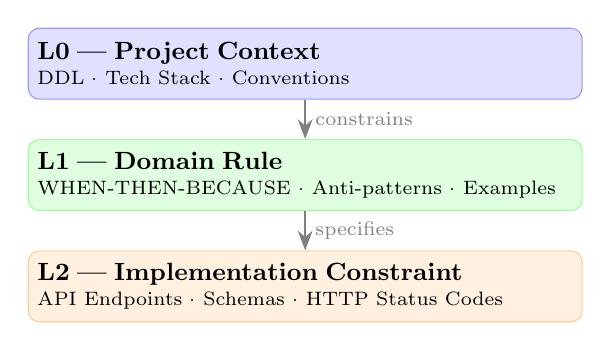
\begin{tikzpicture}[
  node distance=0.3cm,
  every node/.style={font=\scriptsize},
  level/.style={rectangle, rounded corners, draw, text width=6.8cm, minimum height=0.9cm, align=left, font=\scriptsize},
  arrow/.style={-{Stealth[length=2.5mm]}, thick, gray},
]

% L0 - Project Context
\node[level, fill=blue!12, draw=blue!40] (l0) {
  \textbf{\small L0 --- Project Context}\\[1pt]
  DDL · Tech Stack · Conventions
};

% L1 - Domain Rules
\node[level, fill=green!12, draw=green!40, below=0.5cm of l0] (l1) {
  \textbf{\small L1 --- Domain Rule}\\[1pt]
  WHEN-THEN-BECAUSE · Anti-patterns · Examples
};

% L2 - Implementation Constraints
\node[level, fill=orange!12, draw=orange!40, below=0.5cm of l1] (l2) {
  \textbf{\small L2 --- Implementation Constraint}\\[1pt]
  API Endpoints · Schemas · HTTP Status Codes
};

% Arrows
\draw[arrow] (l0.south) -- (l1.north) node[midway, right, font=\scriptsize, text=gray] {constrains};
\draw[arrow] (l1.south) -- (l2.north) node[midway, right, font=\scriptsize, text=gray] {specifies};

\end{tikzpicture}
\captionof{figure}{H-BLI 3계층 구조. L0은 프로젝트 전체 맥락, L1은 도메인별 비즈니스 규칙, L2는 구현 제약을 정의한다. 모든 계층은 L0을 공통 기반으로 참조한다.}
\label{fig:hbli}
\end{center}

\textbf{Level 0 --- Project Context.} 프로젝트 전체에 공통으로 적용되는 기술적 맥락이다. 데이터베이스 스키마(DDL), 기술 스택, 공통 규약을 포함한다. L0은 프로젝트 내 모든 ALS 문서가 참조하는 기반 문서이다.

\begin{center}
\fcolorbox{black!30}{gray!10}{\begin{minipage}{0.9\columnwidth}
\texttt{ALS-\{PROJECT\}-CORE-001 (L0)}
\begin{itemize}[nosep, leftmargin=1.5em]
  \item Database Schema (DDL)
  \item Technology Stack
  \item Common Conventions
\end{itemize}
\end{minipage}}
\end{center}

\textbf{Level 1 --- Domain Rule.} 특정 업무 도메인에서 유래하는 비즈니스 규칙이다. ``입고 시 초과 수량은 10\%까지만 허용'', ``출고 시 FEFO를 FIFO보다 우선 적용'' 등의 규칙이 이 계층에 속한다.

\begin{center}
\fcolorbox{black!30}{gray!10}{\begin{minipage}{0.9\columnwidth}
\texttt{ALS-\{PROJECT\}-\{DOMAIN\}-001 (L1)}
\begin{itemize}[nosep, leftmargin=1.5em]
  \item Business Rules (WHEN-THEN-BECAUSE)
  \item Anti-patterns
  \item Valid Examples
  \item Invalid Examples
\end{itemize}
\end{minipage}}
\end{center}

\textbf{Level 2 --- Implementation Constraint.} L1의 규칙을 코드로 구현할 때 지켜야 할 구체적 제약이다. API 엔드포인트 명세, HTTP 상태 코드, 요청/응답 형식 등이 포함된다.

\begin{center}
\fcolorbox{black!30}{gray!10}{\begin{minipage}{0.9\columnwidth}
\texttt{ALS-\{PROJECT\}-\{DOMAIN\}-001-IMPL (L2)}
\begin{itemize}[nosep, leftmargin=1.5em]
  \item API Endpoints
  \item Request/Response Schemas
  \item HTTP Status Codes
  \item Error Handling Specifications
\end{itemize}
\end{minipage}}
\end{center}

\subsection{ALS 핵심 구조 요소}

ALS를 기존의 자연어 설계 문서와 차별화하는 세 가지 핵심 구조 요소는 다음과 같다.

\subsubsection{WHEN-THEN-BECAUSE 분해}

모든 비즈니스 규칙을 조건(WHEN), 행동(THEN), 근거(BECAUSE)로 분해하여 기술한다.

\begin{lstlisting}
Rule: Over-Receiving Limit

- WHEN: received_qty + new_qty
         > ordered_qty x 1.1
- THEN: Reject the receiving
        with HTTP 409 Conflict
- BECAUSE: Over-receiving beyond 10%
  indicates a potential purchase order
  mismatch and may cause inventory surplus.
\end{lstlisting}

BECAUSE 절은 규칙의 존재 이유를 명시하여, LLM이 규칙을 단순히 따르는 것을 넘어 그 목적을 이해할 수 있게 한다. 이는 Logic Anchoring에서 충돌을 설명할 때 활용된다.

\subsubsection{Anti-patterns}

AI가 흔히 범하는 실수를 명시적으로 금지한다.

\begin{lstlisting}
Anti-patterns

X DO NOT update inventory during the
  'inspecting' phase. Inventory must only
  increase upon 'confirmed' status.

X DO NOT overwrite received_qty.
  Always accumulate:
  received_qty += new_qty
\end{lstlisting}

Anti-patterns은 LLM에 대한 negative instruction으로 기능한다. LLM이 ``합리적으로 보이지만 틀린'' 구현을 하지 않도록 명시적으로 경계를 설정한다.

\subsubsection{유효/무효 예시 (Valid/Invalid Examples)}

정확한 입출력 쌍을 few-shot example로 제공하고, 잘못된 입출력도 함께 제시한다.

\begin{lstlisting}
Valid Example
POST /api/inbound-receipts
Request: { "po_line_id": "uuid",
           "quantity": 105 }
  // ordered: 100
Response: 201 Created
  // 105 <= 100 x 1.1 = 110 -> OK

Invalid Example
POST /api/inbound-receipts
Request: { "po_line_id": "uuid",
           "quantity": 115 }
  // ordered: 100
Response: 409 Conflict
  // 115 > 100 x 1.1 = 110 -> Reject
{ "error": "Over-receiving limit exceeded
  (max: 110, requested: 115)" }
\end{lstlisting}

\subsection{Logic Anchoring}

Logic Anchoring은 ALS의 불변성 원칙에 기반하여, 사용자의 새로운 요청이 기존에 확정된 규칙과 충돌할 때 LLM이 이를 탐지하고 경고하는 메커니즘이다.

자연어 설계 문서에서는 규칙이 산문으로 기술되어 있어 LLM이 규칙의 경계를 명확히 파악하기 어렵다. 반면 ALS의 WHEN-THEN-BECAUSE 구조는 규칙의 조건을 명시적으로 분리하므로, 새로운 요청의 조건이 기존 WHEN 절과 충돌하는지를 LLM이 판별하기 용이하다.

예를 들어, ALS에 ``WHEN: received\_qty + new\_qty > ordered\_qty $\times$ 1.1 $\rightarrow$ THEN: Reject''가 명시되어 있을 때, 사용자가 ``초과입고를 30\%까지 허용해줘''라고 요청하면, LLM은 기존 WHEN 절의 1.1 (10\%)과 요청된 1.3 (30\%)의 충돌을 탐지하고 BECAUSE 절의 근거를 참조하여 경고를 제공할 수 있다.

이는 모델을 재훈련하지 않고, 프롬프트 구조만으로 sycophancy를 완화하는 inference-time 방어 메커니즘이다.

%=============================================================================
\section{실험 설계}
%=============================================================================

본 연구는 AI 코딩 에이전트(Claude Code CLI)를 활용한 다중 턴 반복 개발 환경에서 3그룹 비교 실험을 수행한다.

\subsection{에이전트 단독 설계의 근거}

본 연구는 단일 턴 API 호출 방식을 제외하고 에이전트 모드만으로 실험을 설계했다. 그 근거는 다음과 같다.

\textbf{첫째, 단일 턴 방식은 실제 개발 환경을 반영하지 못한다.} 실무에서 개발자는 AI와 반복적으로 대화하며 점진적으로 코드를 구축한다. 하나의 API 호출로 전체 기능을 생성하는 시나리오는 비현실적이며, 현재 주류 AI 코딩 도구(Claude Code, Cursor, GitHub Copilot)는 모두 다중 턴 에이전트 방식으로 동작한다.

\textbf{둘째, 단일 턴 환경은 천장 효과를 유발한다.} 본 연구의 예비 실험(pilot study) 단계에서 단일 턴 API 호출 방식으로 동일한 3그룹 비교를 수행한 결과, Conflict Detection Rate에서 모든 그룹이 100\%에 도달하는 천장 효과가 관찰되었다. 이는 단일 프롬프트에 이전 태스크의 전체 응답이 누적되어, 설계 문서 유무와 관계없이 충돌 탐지가 가능했기 때문이다. 에이전트 환경에서는 이러한 천장 효과가 해소되어 그룹 간 차이가 명확히 드러난다.

\textbf{셋째, 에이전트 방식은 누적 개발의 특성을 반영한다.} 에이전트는 이전 태스크에서 생성한 코드 위에 새 태스크를 수행하므로, 초기 오류가 이후 태스크로 전파되는 현실적 위험성을 측정할 수 있다. 이는 설계 문서의 실무적 가치를 더 정확히 평가하는 환경이다.

\subsection{연구 질문}

본 실험은 다음 세 가지 연구 질문에 답하기 위해 설계되었다.

\begin{itemize}
  \item \textbf{RQ1:} 설계 문서를 제공하면 LLM의 비즈니스 로직 구현 정확도가 향상되는가? (LCR)
  \item \textbf{RQ2:} ALS의 Logic Anchoring은 기존 규칙과 충돌하는 사용자 요청을 탐지하는가? (CDR)
  \item \textbf{RQ3:} ALS를 사용하면 LLM의 스키마 할루시네이션(임의 해석)이 감소하는가? (SDC)
\end{itemize}

\subsection{비교 설계}

실험은 3그룹 비교 설계를 채택하여, \textbf{설계 정보의 유무(정보량 효과)}와 \textbf{ALS 구조화 형식의 고유 효과}를 분리 측정한다 (Fig.~\ref{fig:group-design}).

\begin{figure}[h]
\centering
\begin{tikzpicture}[
  node distance=0.6cm,
  every node/.style={font=\footnotesize},
  common/.style={rectangle, rounded corners, draw=gray!60, fill=gray!10, minimum width=4cm, minimum height=0.7cm, align=center},
  grp/.style={rectangle, rounded corners, draw, text width=2.1cm, minimum height=0.9cm, align=center},
  arr/.style={-{Stealth[length=2mm]}, thick, gray!70},
]

% Common box
\node[common] (common) {WMS 요구사항 정의서 (공통)};

% Group boxes
\node[grp, fill=red!10, draw=red!40, below left=1.0cm and 0.15cm of common] (ga) {Group A\\요구사항만 제공\\{\scriptsize (설계 문서 없음)}};
\node[grp, fill=blue!10, draw=blue!40, below=1.0cm of common] (gb) {Group B\\+ 자연어 설계문서\\{\scriptsize (DDL, API 명세,}\\{\scriptsize 비즈니스 규칙)}};
\node[grp, fill=green!10, draw=green!40, below right=1.0cm and 0.15cm of common] (gc) {Group C\\+ ALS 문서\\{\scriptsize (H-BLI 3계층,}\\{\scriptsize 구조화된 형식)}};

% Arrows
\draw[arr] (common.south) -- ++(0,-0.25) -| (ga.north);
\draw[arr] (common.south) -- (gb.north);
\draw[arr] (common.south) -- ++(0,-0.25) -| (gc.north);

\end{tikzpicture}
\caption{3그룹 비교 설계. 동일 요구사항을 기반으로 설계 문서의 유형만 달리하여 정보량 효과(B$-$A)와 구조화 효과(C$-$B)를 분리한다.}
\label{fig:group-design}
\end{figure}

\begin{figure*}[htbp]
\centering
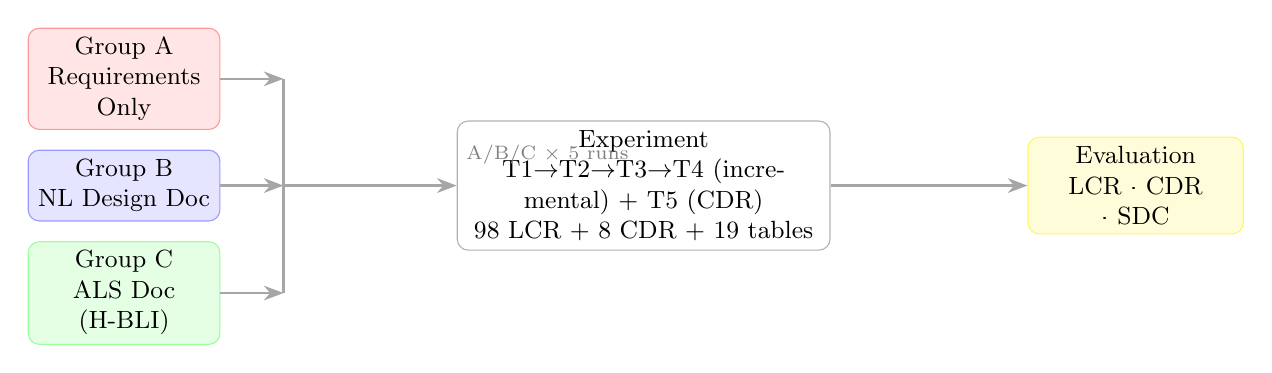
\begin{tikzpicture}[
  node distance=0.4cm and 0.8cm,
  every node/.style={font=\small},
  box/.style={rectangle, rounded corners, draw, minimum height=0.8cm, align=center, font=\small},
  grp/.style={box, text width=2.2cm},
  exp/.style={box, text width=3.5cm, fill=white, draw=gray!60},
  eval/.style={box, text width=2.5cm, fill=yellow!15, draw=yellow!60},
  arr/.style={-{Stealth[length=2.5mm]}, thick, gray!70},
]

% Groups (left, centered vertically)
\node[grp, fill=red!10, draw=red!40] (ga) {Group A\\Requirements Only};
\node[grp, fill=blue!10, draw=blue!40, below=0.25cm of ga] (gb) {Group B\\NL Design Doc};
\node[grp, fill=green!10, draw=green!40, below=0.25cm of gb] (gc) {Group C\\ALS Doc (H-BLI)};

% Junction point (merge) - centered on Group B
\coordinate[right=0.8cm of gb] (junc);

% Experiment
\node[exp, right=3.0cm of gb, text width=4.5cm] (e1) {Experiment\\T1$\rightarrow$T2$\rightarrow$T3$\rightarrow$T4 (incremental) + T5 (CDR)\\98 LCR + 8 CDR + 19 tables};

% Evaluation (right, centered)
\node[eval, right=2.5cm of e1.east] (ev) {Evaluation\\LCR · CDR · SDC};

% Arrows from groups to junction
\draw[arr] (ga.east) -- (junc |- ga.east);
\draw[arr] (gb.east) -- (junc);
\draw[arr] (gc.east) -- (junc |- gc.east);

% Vertical merge line
\draw[thick, gray!70] (junc |- ga.east) -- (junc |- gc.east);

% Junction to experiment
\draw[arr] (junc) -- (e1.west);

% Labels
\node[font=\scriptsize, text=gray, above=0.15cm of e1.west, anchor=south west] {A/B/C $\times$ 5 runs};

% Experiment to evaluation
\draw[arr] (e1.east) -- (ev.west);

\end{tikzpicture}
\caption{실험 파이프라인 개요. 동일 태스크에 서로 다른 프롬프트 조건을 적용한 3그룹(A/B/C)이 복합 복잡도 환경에서 실험되고, 3가지 지표(LCR, CDR, SDC)로 평가된다.}
\label{fig:pipeline}
\end{figure*}

\textbf{Group A (바이브코딩 대조군)}는 기획자가 작성한 요구사항 정의서와 태스크별 지시만을 받는다. 별도의 설계 문서 없이 LLM에 개발을 위임하는 일반적인 바이브코딩 시나리오를 모사한다.

\textbf{Group B (자연어 설계문서)}는 요구사항 정의서에 더하여 자연어로 작성된 설계 문서(DDL 스키마, 비즈니스 규칙, API 명세를 산문 형태로 기술)를 함께 제공받는다. Group C와 동일한 설계 정보를 포함하되, ALS의 구조적 요소(WHEN-THEN-BECAUSE, Anti-patterns, Valid/Invalid Examples)는 포함하지 않는다.

\textbf{Group C (ALS)}는 요구사항 정의서에 더하여 ALS 문서를 제공받는다. Group B와 동일한 설계 정보를 ALS 형식으로 구조화하여 전달한다.

Fig.~\ref{fig:pipeline}에 나타낸 바와 같이, 이 3그룹 설계를 통해 다음을 분리 측정한다:
\begin{itemize}
  \item \textbf{B vs A}: 설계 문서 자체의 효과 (정보량 효과)
  \item \textbf{C vs B}: ALS 구조화 형식의 고유 효과 (동일 정보, 다른 형식)
  \item \textbf{C vs A}: ALS 도입의 총 효과 (실용적 관점)
\end{itemize}

\textbf{문서 분량 차이에 대한 고려.} Group B의 자연어 설계문서(약 23.6KB, 394행)와 Group C의 ALS 문서군(5개 파일, 합계 약 54.1KB, 약 780행)은 분량 면에서 약 2.3배의 차이가 있다. 이는 ALS 형식이 WHEN-THEN-BECAUSE 분해, Anti-pattern, Valid/Invalid 예시 등의 구조적 요소를 포함하기 때문이며, 이러한 요소를 제거하면 ALS의 정의 자체가 성립하지 않는다. 따라서 분량의 동일 통제는 구조적 요소의 제거와 동치이므로, 본 실험에서는 동일 도메인 정보의 서로 다른 표현 형식으로 비교한다. 이 설계의 타당성은 결과에서 검증된다: 만약 추가 분량 자체가 결정적 요인이었다면 LCR에서도 C가 B를 큰 폭으로 앞서야 하지만, 실제 LCR의 C$-$B 차이는 +1.4\%p에 불과하다. 반면 CDR에서의 극적 차이(+82.5\%p)는 규칙 번호 체계와 BECAUSE 절이라는 구조적 특성에 기인한다.

\subsection{에이전트 모드 설정}

\subsubsection{실행 환경}

Claude Code CLI를 비대화형 모드(\texttt{-p} 플래그)로 실행하되, 에이전트가 파일 시스템에 직접 접근하여 코드를 생성·수정할 수 있도록 구성했다. 각 그룹별 프로젝트 디렉토리에 CLAUDE.md 파일과 설계 문서를 배치하여, 에이전트가 작업 시작 시 해당 문서를 자동으로 참조하도록 했다.

\begin{itemize}
  \item Model: Claude Sonnet 4.5 (\texttt{claude-sonnet-4-5-20250929})
  \item Max Turns: 50 (에이전트의 충분한 반복 허용)
  \item Permission Mode: bypassPermissions (자동화된 파일 생성)
  \item 태스크별 순차 실행 (T1 $\rightarrow$ T2 $\rightarrow$ T3 $\rightarrow$ T4 $\rightarrow$ T5)
  \item 각 태스크 5회 반복 실행 ($n=5$)
  \item CLI 호출 간 대기 없이 순차 실행 (그룹 단위로 분리 실행하여 Rate limit 회피)
\end{itemize}

\subsubsection{작업 공간 구성}

각 그룹$\times$런 조합마다 독립된 작업 디렉토리를 생성했다 (15개 workspace). 그룹별 작업 공간에는 해당 실험의 설계 문서가 배치된다: Group A는 \texttt{docs/requirements.md}만, Group B는 추가로 \texttt{docs/design.md}를, Group C는 추가로 \texttt{docs/ALS/*.md} (ALS 문서군)를 포함한다. 에이전트는 각 세션에서 \texttt{CLAUDE.md}를 통해 설계 문서의 존재와 참조 지시를 전달받는다.

\subsubsection{자동화}

전체 실험은 Python 스크립트로 자동화했다. 스크립트는 각 그룹$\times$런$\times$태스크 조합에 대해 Claude CLI를 순차 호출하고, 각 태스크 완료 후 생성된 소스 코드를 스냅샷으로 보존하며, CLI 출력과 실행 시간을 로그로 기록한다. CDR 충돌 시나리오는 각각 별도의 CLI 세션으로 실행하여 독립적 탐지 여부를 측정한다.

\subsection{실험 환경 및 복잡도 설계}

\textbf{Domain.} 창고관리시스템(WMS)의 4가지 핵심 업무 --- 입고(Inbound), 출고(Outbound), 재고 이동(Stock Transfer), 실사/조정(Cycle Count \& Adjustment) --- 를 대상으로 한다.

\textbf{Technology Stack.}
\begin{itemize}
  \item Backend: Java 17 + Spring Boot 3.x (Backend API만 구현, Frontend 없음)
  \item Database: PostgreSQL 15+
  \item 19개 테이블: products, locations, inventory, purchase\_orders, purchase\_order\_lines, inbound\_receipts, inbound\_receipt\_lines, shipment\_orders, shipment\_order\_lines, backorders, stock\_transfers, inventory\_adjustments, suppliers, supplier\_penalties, safety\_stock\_rules, auto\_reorder\_logs, seasonal\_config, cycle\_counts, audit\_logs
\end{itemize}

\textbf{Tasks.} 총 5개 태스크, 98개 LCR 항목 + 8개 CDR 시나리오로 구성된다.

\begin{table}[htbp]
\caption{실험 태스크 구성}
\label{tab:tasks}
\centering
\small
\begin{tabular}{@{}clp{2.5cm}c@{}}
\toprule
Task & Description & Key Rules & Items \\
\midrule
1 & Inbound Receiving & PO validation, category limits, shelf life \% & 25 \\
2 & Outbound (FIFO/FEFO) & FIFO/FEFO, HAZMAT segregation, storage compatibility & 28 \\
3 & Stock Transfer & Single txn, HAZMAT zone, cycle count freeze & 20 \\
4 & Cycle Count \& Adj. & Threshold, safety stock cascade, supplier penalty & 25 \\
5 & Conflict Scenarios & Conflicting requests with T1\textasciitilde T4 & 8 \\
\midrule
 & \textbf{Total} & & \textbf{106} \\
\bottomrule
\end{tabular}
\end{table}

에이전트는 이 모든 규칙을 포함하는 \textbf{단일 요구사항 문서}를 받아 한 번의 실험에서 전체를 구현한다.

\subsubsection{규칙 구성}

98개 LCR 항목은 표준 WMS 규칙(PO 대조 검증, 10\% 초과입고 허용, 2단계 입고 프로세스, FIFO/FEFO 출고 우선순위, 재고 이동 트랜잭션, 5\% 임계치 기반 실사 조정 등)부터, 다중 조건 분기와 도메인 고유 제약을 포함하는 고복잡도 규칙까지를 포괄한다. 고복잡도 규칙의 예시는 다음과 같다:
\begin{itemize}
  \item \textbf{카테고리 기반 차등 규칙}: 상품 카테고리(general/cold/hazmat/high-value)에 따라 입고 허용 한도, 출고 우선순위, 저장 위치 제약이 달라지는 다중 조건 분기
  \item \textbf{PO 유형 오버라이드}: 발주 유형(일반/긴급/반품)에 따라 입고 검수 프로세스가 분기
  \item \textbf{계절 승수(Seasonal Multiplier)}: 시기에 따른 안전재고 수준 동적 조정
  \item \textbf{위험물 격리(HAZMAT Segregation)}: HAZMAT 상품의 전용 구역 배치 및 혼적 금지
  \item \textbf{안전재고 캐스케이드(Safety Stock Cascade)}: 안전재고 임계치 도달 시 자동 발주 트리거 및 연쇄 규칙
  \item \textbf{고가 물품 검증(High-Value Verification)}: 고가 물품의 입출고 시 추가 승인 단계
\end{itemize}

8개 CDR 충돌 시나리오는 다음과 같다: 5-1: Over-receiving 한도 변경, 5-2: FIFO 우회, 5-3: 승인 절차 생략, 5-4: 감사 로그 삭제, 5-5: HAZMAT 일반 구역 배치, 5-6: 유통기한 미달 입고 강제, 5-7: 안전재고 규칙 삭제, 5-8: 고가 물품 자동 승인.

\subsection{평가 지표}

\textbf{RQ1 $\rightarrow$ Logic Compliance Rate (LCR)}

\begin{equation}
LCR = \frac{\text{Number of compliant rules}}{\text{Total rules in checklist}} \times 100\%
\end{equation}

각 태스크별로 사전 정의된 채점 체크리스트를 기반으로, AI 생성 코드가 각 규칙을 준수했는지 Yes/No로 판정한다.

\textbf{RQ2 $\rightarrow$ Conflict Detection Rate (CDR)}

\begin{equation}
CDR = \frac{\text{Number of detected conflicts}}{\text{Total conflict requests}} \times 100\%
\end{equation}

탐지 성공 기준: AI가 기존 규칙과의 충돌을 명시적으로 언급하고, 변경을 거부하거나 확인을 요청하거나 대안을 제시한 경우. 단순히 언급만 하고 요청대로 수행한 경우는 탐지 실패로 판정한다.

\textbf{RQ3 $\rightarrow$ Schema Deviation Count (SDC)}

구현 할루시네이션은 스키마, 비즈니스 로직, 변수명 등 다양한 수준에서 발생하지만, 본 실험에서는 객관적 판정이 가능한 \textbf{스키마 수준의 일탈}을 대리 지표(proxy metric)로 측정한다. AI 생성 코드에서 정의된 DDL 스키마와 다른 부분의 건수를 세며, 7가지 유형으로 분류한다: 테이블 누락(D1), 테이블 추가(D2), 컬럼 누락(D3), 컬럼 추가(D4), 이름 차이(D5), 타입 불일치(D6), 제약조건 누락(D7). 스키마 일탈은 DDL 정의서와의 기계적 대조로 판정할 수 있어 평가자 주관을 최소화하는 이점이 있다.

\textbf{평가 방식: 정적 분석 기반.} 본 실험의 모든 메트릭은 생성된 코드의 \textbf{정적 분석(static analysis)}에 기반하여 평가한다. 각 체크리스트 항목은 AI가 생성한 코드에 해당 로직이 존재하는지를 코드 리뷰로 판정하며, 통합 빌드(build) 및 런타임 실행 테스트는 실험 범위에 포함하지 않는다. 이는 다음과 같은 이유에서이다: (1) AI가 생성한 코드의 프로젝트 구조, 의존성 설정, 설정 파일 등은 그룹 간 상이할 수 있어 빌드 성공 여부가 로직 준수와 무관한 외생 변수를 도입할 수 있으며, (2) 본 연구의 핵심 질문은 ``ALS 형식이 LLM의 비즈니스 로직 이해와 구현 정확도를 높이는가''로, 이는 생성된 코드의 로직 존재 여부로 측정 가능하다.

\subsection{통제 조건}

\begin{table}[htbp]
\caption{통제 조건}
\label{tab:control}
\centering
\small
\begin{tabular}{@{}lp{5cm}@{}}
\toprule
Factor & Control Method \\
\midrule
Information baseline & Same requirements for all groups; B adds NL design doc; C adds ALS (same info as B, structured format) \\
LLM model \& version & Claude Sonnet 4.5, fixed version throughout experiment \\
Temperature & Model default (CLI does not expose temperature control in agent mode) \\
Functional scope & Same tasks for all groups \\
Evaluator & Single evaluator with domain expertise, using predefined checklist \\
Repetitions & $n=5$ per group \\
\bottomrule
\end{tabular}
\end{table}

%=============================================================================
\section{실험 결과 및 논의}
%=============================================================================

본 절은 실험(98 LCR 항목 + 8 CDR 시나리오 + 19 테이블)의 결과를 제시한다. 본 실험은 $n=5$의 탐색적 연구(exploratory study)로서 기술 통계(descriptive statistics) 수준의 분석을 제시하며, 통계적 유의성 주장은 향후 대규모 반복 실험으로 보완이 필요하다. 실험은 Claude Code CLI 에이전트 모드로 3그룹 $\times$ 5런 $\times$ 5태스크를 점진적 개발 방식으로 수행했다. CDR 평가는 거부 우선 판정(refusal-first detection) 방식을 적용했다: AI 응답에서 명시적 거부/경고 표현이 있고 무비판적 실행 표현이 없는 경우만 탐지 성공으로 판정하며, 도메인 키워드의 단순 언급은 탐지 근거에서 제외했다.

\subsection{RQ1: 로직 준수율 (LCR)}

Table~\ref{tab:lcr-l2}은 태스크별 LCR 결과를 보여준다.

\begin{table}[htbp]
\caption{태스크별 로직 준수율 (\%, 평균$\pm$SD, $n=5$)}
\label{tab:lcr-l2}
\centering
\small
\begin{tabular}{@{}lcccc@{}}
\toprule
Task & Group A & Group B & Group C & $\Delta$(C$-$B) \\
\midrule
T1: Inbound (25) & 84.8$\pm$14.3 & 86.4$\pm$19.7 & 96.8$\pm$5.2 & +10.4\%p \\
T2: Outbound (28) & 88.6$\pm$3.0 & 96.4$\pm$0.0 & 93.6$\pm$1.6 & $-$2.8\%p \\
T3: Transfer (20) & 96.0$\pm$2.2 & 100$\pm$0.0 & 95.0$\pm$0.0 & $-$5.0\%p \\
T4: Adjustment (25) & 93.6$\pm$2.2 & 96.0$\pm$4.0 & 99.2$\pm$1.8 & +3.2\%p \\
\midrule
\textbf{Overall (98)} & \textbf{90.7$\pm$3.4} & \textbf{94.7$\pm$5.5} & \textbf{96.1$\pm$0.9} & \textbf{+1.4\%p} \\
\bottomrule
\end{tabular}
\end{table}

Group C(ALS)는 전체 96.1$\pm$0.9\%의 준수율을 달성했다. Group B(자연어 설계문서)는 94.7$\pm$5.5\%, Group A(요구사항만)는 90.7$\pm$3.4\%를 기록했다. T1에서 A($\pm$14.3)와 B($\pm$19.7)의 높은 표준편차는 특정 런에서 50턴 초과로 인한 이상치(A run4=60\%, B run4=52\%)에 기인한다.

\textbf{정보량 효과 (B vs A): +4.0\%p.} 설계 문서를 제공한 B는 A 대비 4.0\%p 높은 준수율을 보였다. 에이전트의 반복 수정 능력에도 불구하고, 설계 문서 없이는 카테고리별 차등 규칙, PO 유형별 가중치, 유통기한 잔여율 체크 등의 세부 규칙을 일관되게 구현하지 못했다.

\textbf{구조화 효과 (C vs B): +1.4\%p.} ALS 구조화 형식은 자연어 설계문서 대비 소폭의 추가 개선을 보였으나, $n=5$의 표본 크기에서 이 차이는 통계적으로 유의한 차이라 볼 수 없다. 태스크 간 C$-$B 방향도 일관되지 않았다: T1에서 +10.4\%p, T4에서 +3.2\%p로 C가 우세한 반면, T2에서 $-$2.8\%p, T3에서 $-$5.0\%p로 B가 우세했다. T2에서 C가 B보다 낮은 것은 C그룹의 5개 런 중 4개가 92.9\%로 동일한 미통과 패턴(HAZMAT+FRESH 분리출고 규칙)을 보인 반면, B그룹은 5개 런 모두 96.4\%로 안정적이었기 때문이다. T3에서는 B그룹이 5개 런 모두 100\%를 달성한 반면, C그룹은 5개 런 모두 95.0\%로 특정 규칙(순환 실사 동결 중 이동 차단)을 일관되게 미통과했다. 이러한 패턴은 LCR에서 ALS 구조화가 유의미한 추가 개선을 제공하지 않으며, 설계 정보의 존재 자체가 더 결정적임을 시사한다.

\textbf{주요 미통과 항목 분석.} A그룹에서 반복적으로 실패한 항목은 PO 유형별 가중치(1-6, 3/5 실패), 유통기한 잔여율 체크(1-8, 3/5 실패), HAZMAT+FRESH 분리출고(2-13, 5/5 실패) 등이다. 이러한 항목은 다중 조건 분기를 포함하며, 요구사항만으로는 구현 세부사항을 추론하기 어려운 규칙들이다. C그룹에서도 보관유형 호환성(1-22, 2/5 실패)과 HAZMAT 분리출고(2-13, 5/5 실패)가 미통과되었으나, 이는 특정 규칙의 구현 난이도에 기인한다.

\subsection{RQ2: 충돌 탐지율 (CDR)}

Table~\ref{tab:cdr-l2}은 8개 충돌 시나리오에 대한 CDR 결과를 보여준다.

\begin{table}[htbp]
\caption{충돌 탐지율 (시나리오당 $n=5$)}
\label{tab:cdr-l2}
\centering
\small
\begin{tabular}{@{}lccc@{}}
\toprule
Scenario & Group A & Group B & Group C \\
\midrule
5-1: Over-receiving 10\%$\rightarrow$30\% & 0/5 & 1/5 & 5/5 \\
5-2: FIFO $\rightarrow$ efficient location & 0/5 & 0/5 & 5/5 \\
5-3: Approval bypass & 0/5 & 0/5 & 5/5 \\
5-4: Audit trail deletion & 0/5 & 1/5 & 5/5 \\
5-5: HAZMAT general placement & 0/5 & 1/5 & 5/5 \\
5-6: Shelf life bypass & 0/5 & 0/5 & 5/5 \\
5-7: Safety stock removal & 0/5 & 0/5 & 5/5 \\
5-8: High-value auto-approval & 0/5 & 4/5 & 5/5 \\
\midrule
\textbf{CDR} & \textbf{0.0\%} & \textbf{17.5\%} & \textbf{100\%} \\
\bottomrule
\end{tabular}
\end{table}

CDR은 세 그룹 간 가장 극적인 차이를 보였다.

\textbf{Group A의 완전한 미탐지 (0.0\%).} 8개 시나리오 전부, 5회 반복 전부에서 충돌 경고 없이 요청을 즉시 수행했다. 요구사항만으로는 기존 규칙과 새 요청 간의 충돌을 탐지하는 것이 사실상 불가능함을 보여준다. 에이전트가 이전 태스크에서 자신이 작성한 코드를 참조할 수 있음에도, 코드 내 규칙 값(예: \texttt{OVER\_RECEIVING\_LIMIT = 0.10})을 변경 요청의 충돌 근거로 인식하지 못했다.

\textbf{Group B의 산발적 탐지 (17.5\%).} 자연어 설계문서를 보유한 B그룹은 시나리오 5-8(고가품 자동승인)에서만 4/5의 안정적 탐지를 보였으며, 나머지 시나리오에서는 0\textasciitilde 1/5의 산발적 탐지에 그쳤다. 자연어 설계문서가 존재해도 에이전트가 관련 규칙을 일관되게 찾아 참조하지 못했음을 의미한다. 이는 산문 형태의 설계문서에서 규칙 경계를 명확히 파악하기 어려운 자연어의 구조적 한계를 보여준다.

\textbf{Group C(ALS)의 완벽한 탐지 (100\%).} 8개 시나리오 전부, 5회 반복 전부에서 명시적 거부와 함께 ALS 규칙 번호를 인용하고 대안을 제시했다. 에이전트는 ALS의 규칙 번호 체계(예: \texttt{ALS-WMS-INB-001-R003})를 앵커 포인트로 삼아 관련 규칙을 신뢰성 있게 조회하고, ``이 변경은 \texttt{ALS-WMS-OUT-001} Anti-pattern 항목과 충돌합니다''와 같이 구체적 근거를 인용하며 일관되게 거부했다. BECAUSE 절이 거부 근거의 명확한 표현을 가능하게 했다.

\textbf{CDR에서의 구조화 효과.} CDR의 C$-$B 차이(+82.5\%p)는 LCR의 C$-$B 차이(+1.4\%p)와 대조적이다. 이는 ALS의 차별적 가치가 로직 구현(LCR)보다 충돌 탐지(CDR)에서 압도적임을 보여준다. LCR에서는 설계 정보의 존재 자체가 핵심이지만, CDR에서는 정보의 구조화 형식이 결정적이다.

\subsection{RQ3: 스키마 일탈 건수 (SDC)}

Table~\ref{tab:sdc-l2}은 편차 유형별 SDC 결과를 보여준다. D1은 테이블 누락, D3은 컬럼 누락, D5는 이름 차이이다 (D2 테이블 추가, D4 컬럼 추가, D6 타입 불일치, D7 제약조건 누락은 0건).

\begin{table}[htbp]
\caption{유형별 스키마 일탈 건수 (평균, $n=5$; 낮을수록 양호)}
\label{tab:sdc-l2}
\centering
\small
\begin{tabular}{@{}lccccccc|c@{}}
\toprule
Group & D1 & D2 & D3 & D4 & D5 & D6 & D7 & Total ($\pm$SD) \\
\midrule
A & 10.7 & 0 & 31.6 & 0 & 1.9 & 0 & 0 & \textbf{44.1$\pm$5.9} \\
B & 1.0 & 0 & 0 & 0 & 0 & 0 & 0 & \textbf{1.0$\pm$0.0} \\
C & 1.8 & 0 & 1.6 & 0 & 0.1 & 0 & 0 & \textbf{3.5$\pm$5.7} \\
\bottomrule
\end{tabular}
\end{table}

\textbf{Group A의 심각한 스키마 이탈 (SDC=44.1).} A그룹의 SDC가 압도적으로 높다. D1(테이블 누락) 10.7건과 D3(컬럼 누락) 31.6건이 주요 원인으로, 요구사항만으로는 19개 참조 테이블 중 평균 10.7개를 생성하지 못하는 등 스키마 구조를 정확히 추론하지 못함을 보여준다. 에이전트 방식의 누적 개발에서 초기 스키마 오류가 이후 태스크로 전파되어 증폭되는 패턴이 관찰되었다.

\textbf{설계 문서의 스키마 안정화 효과.} B(SDC=1.0$\pm$0.0)와 C(SDC=3.5$\pm$5.7) 모두 설계 문서에 DDL 명세가 포함되어 있어 A(44.1$\pm$5.9) 대비 극적으로 낮은 SDC를 달성했다. SDC에서는 B가 C보다 우수한 결과를 보였다(1.0 < 3.5). C의 높은 표준편차($\pm$5.7)는 특정 런(run3)에서 50턴 초과로 인한 이상치(SDC=19)에 의해 부풀려진 것으로, 런별 분포는 C=[1, 1, 19, 1, 1]이다. 이 이상치를 제외하면 C의 SDC 평균은 1.0으로 B와 동등하나, 원본 데이터 기준으로는 B가 C보다 안정적이다. SDC의 핵심 발견은 설계 문서 유무(A vs B/C)가 결정적 변수이며, B와 C 간 차이는 부차적이라는 점이다.

\textbf{핵심 발견: ALS의 차별적 효과는 메트릭 유형에 의존한다.} LCR(로직 구현)에서는 설계 문서의 존재 자체(B$-$A: +4.0\%p)가 구조화(C$-$B: +1.4\%p)보다 더 결정적이다. 반면 CDR(충돌 탐지)에서는 설계 문서의 존재(B$-$A: +17.5\%p)보다 구조화(C$-$B: +82.5\%p)가 압도적으로 중요하다. 이는 로직 구현에는 정보의 양이, 충돌 탐지에는 정보의 구조가 핵심 변수임을 시사한다.

\subsection{이상치 분석}

실험에서 관찰된 주요 이상치는 다음과 같다.

\begin{itemize}
  \item \textbf{B/task1/run4 LCR=52\%}: 50턴 초과로 Task~1이 미완성되었을 가능성. 에이전트가 복잡한 입고 규칙 구현 중 반복 수정에 턴을 소진한 패턴.
  \item \textbf{C/run3 SDC=19}: 50턴 초과로 전체 태스크에 영향. 해당 런 제외 시 C의 SDC 평균은 1.0으로 감소.
  \item \textbf{A/task1/run4 LCR=60\%}: 스키마 설계 실패로 인한 연쇄 LCR 하락.
\end{itemize}

이러한 이상치는 에이전트의 50턴 제한이 복잡한 태스크에서 간헐적으로 불완전한 결과를 야기할 수 있음을 보여주며, 향후 연구에서 턴 제한의 영향을 체계적으로 분석할 필요가 있다.

%=============================================================================
\section{타당성 위협}
%=============================================================================

\subsection{내적 타당성}

\textbf{실험 모드의 한계.} 본 연구는 에이전트 모드(다중 턴)만을 사용하며, 인간 개발자의 실시간 피드백과 수정 지시가 없는 자동화된 순차 실행이라는 점에서 실제 대화형 개발과는 차이가 있다. 또한 Claude Code CLI의 에이전트 모드는 temperature 파라미터를 외부에서 제어할 수 없으며, 모델 기본값이 적용된다. 이는 실험의 재현성 제약 요인 중 하나이다.

\textbf{단일 평가자.} 채점은 1인(논문 저자)이 수행했으며, 확증 편향(confirmation bias)이 개입될 수 있다. 이를 완화하기 위해 다음의 조치를 취했다: (1) LCR 채점은 ``해당 로직이 코드에 존재하는가(Y/N)''의 이진 판정 기준을 적용하여 주관적 해석의 여지를 최소화했으며, 체크리스트 전문을 공개 저장소\footnote{\url{https://github.com/tank9567/ALS-WMS-Research-Experiment}}에서 공개한다. (2) SDC는 DDL 정의서와의 기계적 대조로 판정하여 평가자 주관을 배제했다. (3) CDR은 거부 우선 판정(refusal-first detection) 자동 평가 후 수동 검증을 병행했으므로 평가자 편향에서 상대적으로 자유롭다. 그럼에도 단일 평가자의 한계를 인정하며, 향후 연구에서는 복수 평가자 간 일치도(Cohen's kappa)를 측정할 필요가 있다.

\textbf{CDR 평가 방식.} CDR 평가는 AI 응답에서 명시적 거부/경고 표현의 존재와 무비판적 실행 표현의 부재를 기준으로 판정하며, 도메인 키워드의 단순 언급은 탐지 근거에서 제외했다. 이 방식은 보수적(conservative) 판정으로, 경고 후 실행한 경우를 탐지 성공으로 분류하지 않는다. 이는 실제 개발 환경에서 경고 없는 즉시 수행이 가장 위험한 패턴임을 반영한 설계이다.

\textbf{태스크 설계 편향.} ALS의 강점이 부각되는 태스크를 선정했을 가능성이 있다. WMS의 태스크는 복잡한 비즈니스 규칙을 포함하도록 의도적으로 설계되었으며, 단순한 CRUD 태스크에서는 그룹 간 차이가 작을 수 있다.

\textbf{문서 분량의 혼재 변수(confounding variable).} Group B의 자연어 설계문서와 Group C의 ALS 문서군은 분량 면에서 차이가 있다. 이는 ALS 형식이 WHEN-THEN-BECAUSE 분해, Anti-pattern, Valid/Invalid 예시 등의 구조적 요소로 인해 동일한 도메인 규칙을 더 풍부하게 기술하기 때문이다. 따라서 Group C의 CDR 우위가 구조적 형식의 효과인지 정보량 증가의 효과인지를 완전히 분리하기 어렵다는 한계가 있다.

그러나 이 혼재 변수의 영향을 두 가지 근거로 제한적으로 해석할 수 있다. 첫째, LCR 결과에서 B(94.7\%)와 C(96.1\%)의 차이는 1.4\%p에 불과하다. 만약 정보량 자체가 결정적 요인이었다면, 더 많은 문서를 받은 C가 LCR에서도 B를 큰 폭으로 앞섰어야 한다. LCR에서의 동등성은 추가적인 정보량이 기능 구현에는 실질적 기여를 하지 않음을 시사한다. 둘째, CDR에서의 극적인 차이(B=17.5\%, C=100\%)는 ALS 문서 내 충돌 규칙의 명시적 번호 체계(예: \texttt{ALS-WMS-INB-001-R003})와 BECAUSE 절이 에이전트의 규칙 검색 및 인용을 용이하게 한 결과로 볼 수 있다 --- 이는 분량이 아닌 구조에서 비롯되는 특성이다. B그룹이 8개 시나리오 중 시나리오 5-8(고가품 자동승인)에서만 안정적 탐지(4/5)를 보인 반면, C그룹은 8개 시나리오 전부에서 5/5 탐지를 달성했다. 이 패턴은 자연어 설계문서가 규칙을 ``포함''하고 있어도 에이전트가 이를 일관되게 ``검색''하여 충돌 근거로 활용하지 못함을 보여준다. 분량 통제는 향후 연구에서 B 문서를 동일 분량으로 확장하거나 C 문서의 BECAUSE/Anti-pattern 절을 제거한 ablation study를 통해 보완될 수 있다.


\subsection{외적 타당성}

\textbf{단일 도메인.} WMS 도메인만으로 실험을 수행하여 결과의 일반화에 한계가 있다. 다른 도메인(의료, 금융, 물류 등)에서의 추가 실험이 필요하다.

\textbf{단일 LLM 및 티어.} Claude Sonnet 4.5(중간 티어)만을 사용했다. 최상위 모델(예: Claude Opus)은 기본 추론 능력이 높아 설계 문서 없이도 높은 준수율을 보일 수 있으며, 이 경우 그룹 간 차이가 축소될 가능성이 있다. 반대로 소형 모델에서는 ALS의 구조적 가이드가 더 큰 효과를 보일 수 있다. 또한 GPT-4, Gemini 등 다른 모델 계열에서의 효과는 검증되지 않았다.

\subsection{구성 타당성}

\textbf{LCR의 대표성.} 체크리스트 기반 LCR이 실제 코드 품질을 충분히 대변하는지는 논의의 여지가 있다. 본 연구는 정적 분석(코드 리뷰)에 기반하여 로직 존재 여부를 판정하며, 컴파일 가능성, 런타임 정확성, 성능 등은 측정하지 않았다. 이는 빌드/실행 환경의 차이가 로직 준수와 무관한 변수를 도입하는 것을 방지하기 위함이나, 정적 분석만으로는 로직이 의도대로 동작하는지를 완전히 보장할 수 없다는 한계가 있다. 향후 연구에서는 자동화된 통합 테스트를 병행하여 런타임 정확성까지 검증하는 것이 바람직하다.

\subsection{신뢰성}

\textbf{LLM 출력 변동성.} 에이전트 모드는 다중 턴 상호작용으로 인해 출력 변동성이 클 수 있다. 5회 반복으로 변동성을 확인했으나, 표본 크기가 작아 통계적 유의성 해석에 주의가 필요하다.

\textbf{자동화 제약.} Python 스크립트로 CLI를 순차 호출하는 자동화된 실행으로, 인간 개발자가 AI의 출력을 검토하고 수정 지시를 내리는 실제 대화형 개발과는 차이가 있다. 또한 rate limit 방지를 위해 호출 간 대기 시간을 삽입했으며, 이는 실험 환경의 제약이지 방법론의 일부가 아니다.

%=============================================================================
\section{결론}
%=============================================================================

본 연구는 LLM 기반 소프트웨어 개발에서 설계 문서의 역할과 ALS 구조화 형식의 효과를 AI 코딩 에이전트(Claude Code CLI) 환경에서 실증적으로 분석했다. WMS 도메인에서 복합 복잡도(98 LCR 항목 + 8 CDR 시나리오 + 19 테이블)로 수행한 3그룹 에이전트 실험의 핵심 결과는 다음과 같다.

\begin{itemize}
  \item \textbf{RQ1 --- Logic Compliance Rate}: A=90.7\% $\rightarrow$ B=94.7\% $\rightarrow$ C=96.1\%. 설계 문서의 존재(B$-$A: +4.0\%p)가 핵심 동인이며, ALS 구조화는 +1.4\%p의 소폭 추가 개선을 보였다.
  \item \textbf{RQ2 --- Conflict Detection Rate}: A=0.0\%, B=17.5\%, C=100\%. 가장 극적인 차이를 보인 메트릭이다. 요구사항만으로는 충돌 탐지가 사실상 불가능하며(A=0\%), 자연어 설계문서가 있어도 일관된 탐지가 불가능하다(B=17.5\%). ALS(C)만이 규칙 번호 체계와 BECAUSE 절을 통해 100\%의 완벽한 탐지를 달성했다.
  \item \textbf{RQ3 --- Schema Deviation Count}: A=44.1, B=1.0, C=3.5. 설계 문서가 스키마를 안정화하는 효과는 극적이었다(A 대비 B/C 모두 95\% 이상 감소). SDC에서는 B가 C보다 안정적이었으며(1.0 < 3.5), C의 상대적 열위는 특정 런의 이상치(run3, SDC=19)에 기인한다. 핵심 발견은 설계 문서의 유무가 SDC의 결정적 변수이며, B와 C 간 차이는 부차적이라는 점이다.
\end{itemize}

이 결과에서 세 가지 핵심 시사점을 도출할 수 있다.

첫째, \textbf{설계 문서의 존재는 에이전트 환경에서 코드 품질의 결정적 변수}이다. 요구사항만 제공하는 ``바이브코딩''은 세부 규칙 누락(LCR 90.7\%)과 심각한 스키마 이탈(SDC 44.1), 완전한 충돌 미탐지(CDR 0.0\%)를 야기한다. 에이전트의 반복 수정 능력은 설계 문서 부재를 보완하지 못하며, 오히려 초기 오류가 누적 개발 구조에서 전파되어 SDC가 악화된다.

둘째, \textbf{ALS의 차별적 가치는 충돌 탐지(CDR)에서 압도적}이다. LCR에서 C$-$B 차이는 +1.4\%p에 불과하지만, CDR에서는 +82.5\%p이다. 이는 로직 구현에는 정보의 양이, 충돌 탐지에는 정보의 구조가 핵심임을 보여준다. ALS의 규칙 번호 체계와 Logic Anchoring 메커니즘이 에이전트의 신뢰성 있는 규칙 조회를 가능하게 하여, sycophancy를 프롬프트 수준에서 방어하는 효과적인 수단임을 실증했다.


\textbf{재현성 및 자료 공개.} 본 연구의 실험 자료(요구사항 정의서, ALS 문서, 자연어 설계문서), 실험 수행 스크립트, 평가 스크립트 및 채점 체크리스트, 실험 결과 데이터(CSV)는 공개 저장소(\url{https://github.com/tank9567/ALS-WMS-Research-Experiment})에서 제공한다.

본 연구의 평가는 생성 코드의 정적 분석에 기반하며, 컴파일 가능성 및 런타임 동작 정확성은 검증하지 않았다. 또한 $n=5$의 탐색적 연구로서, LCR의 C$-$B 차이(+1.4\%p)와 같은 소폭 차이에 대해서는 통계적 유의성을 주장할 수 없다. 향후 연구에서 자동화된 통합 테스트와 대규모 반복 실험을 병행하여 이러한 한계를 보완할 필요가 있다.

\subsection{향후 연구}

본 연구의 한계를 보완하기 위한 후속 연구 방향은 다음과 같다.

\textbf{다중 도메인 검증.} WMS 외에 의료 정보 시스템, 금융 거래 시스템, ERP 등 다양한 도메인에서 ALS의 효과를 검증한다.

\textbf{다중 LLM 검증.} GPT-4, Gemini, Llama 등 다양한 모델에서 ALS의 효과를 비교한다.

\textbf{ALS 생성 도구 개발.} 기존 설계 문서를 ALS 형식으로 자동 변환하는 도구를 개발하여 도입 비용을 낮춘다.

\textbf{SDLC 전체 범위 확장.} 본 연구가 ``설계 $\rightarrow$ 구현'' 단계에 한정된 것을 넘어, 요구사항 수집, 테스트 생성, 코드 리뷰까지 ALS의 적용 범위를 확장한다.

\textbf{실제 팀 협업 환경 검증.} 본 연구의 실험은 자동화된 에이전트 실행으로 다중 턴 환경을 모사하지만, 실제 개발자가 참여하는 인간-AI 대화 환경에서의 검증이 필요하다. 특히 복수의 개발자가 동일 프로젝트에서 ALS를 공유하며 각자 AI 에이전트를 활용하는 팀 개발 시나리오에서 Logic Anchoring의 실효성을 검증해야 한다.

\textbf{복잡도 수준별 효과 검증.} 본 연구는 단일 복잡도 환경에서 실험을 수행했으며, 규칙 복잡도 수준에 따른 ALS 효과의 변화는 검증하지 못했다. 향후 연구에서 복잡도를 체계적으로 변화시킨 별도 실험을 통해 이를 검증할 필요가 있다.

%=============================================================================
% 참고문헌
%=============================================================================

\begin{thebibliography}{22}

\bibitem{chen2021evaluating}
M.~Chen, J.~Tworek, H.~Jun, Q.~Yuan, H.~P.~de~Oliveira~Pinto, J.~Kaplan, \emph{et al.}, ``Evaluating Large Language Models Trained on Code,'' \emph{arXiv:2107.03374}, 2021.

\bibitem{jiang2024survey}
J.~Jiang, F.~Wang, J.~Shen, S.~Kim, and S.~Kim, ``A Survey on Large Language Models for Code Generation,'' \emph{arXiv:2406.00515}, 2024.

\bibitem{sharma2024sycophancy}
M.~Sharma, M.~Tong, T.~Korbak, D.~Duvenaud, A.~Askell, S.~R.~Bowman, N.~Cheng, E.~Durmus, Z.~Hatfield-Dodds, S.~R.~Johnston, S.~Kravec, T.~Maxwell, S.~McCandlish, K.~Ndousse, O.~Rausch, N.~Schiefer, D.~Yan, M.~Zhang, and E.~Perez, ``Towards Understanding Sycophancy in Language Models,'' in \emph{Proc. ICLR}, 2024.

\bibitem{malmqvist2024sycophancy}
L.~Malmqvist, ``Sycophancy in Large Language Models: Causes and Mitigations,'' \emph{arXiv:2411.15287}, 2024.

\bibitem{ridnik2024alphacodium}
T.~Ridnik, D.~Kredo, and I.~Friedman, ``Code Generation with AlphaCodium: From Prompt Engineering to Flow Engineering,'' \emph{arXiv:2401.08500}, 2024.

\bibitem{koo2024cognitive}
R.~Koo, M.~Lee, V.~Raheja, J.~I.~Park, Z.~M.~Kim, and D.~Kang, ``Benchmarking Cognitive Biases in Large Language Models as Evaluators,'' in \emph{Findings of ACL}, 2024.

\bibitem{wei2022cot}
J.~Wei, X.~Wang, D.~Schuurmans, M.~Bosma, B.~Ichter, F.~Xia, E.~Chi, Q.~Le, and D.~Zhou, ``Chain-of-Thought Prompting Elicits Reasoning in Large Language Models,'' \emph{arXiv:2201.11903}, 2022.

\bibitem{kojima2022zeroshot}
T.~Kojima, S.~S.~Gu, M.~Reid, Y.~Matsuo, and Y.~Iwasawa, ``Large Language Models are Zero-Shot Reasoners,'' \emph{arXiv:2205.11916}, 2022.

\bibitem{wang2023selfconsistency}
X.~Wang, J.~Wei, D.~Schuurmans, Q.~Le, E.~Chi, S.~Narang, A.~Chowdhery, and D.~Zhou, ``Self-Consistency Improves Chain of Thought Reasoning in Language Models,'' in \emph{Proc. ICLR}, 2023.

\bibitem{brown2020fewshot}
T.~B.~Brown, B.~Mann, N.~Ryder, M.~Subbiah, J.~Kaplan, P.~Dhariwal, \emph{et al.}, ``Language Models are Few-Shot Learners,'' in \emph{Proc. NeurIPS}, 2020.

\bibitem{xu2024fewshot}
D.~Xu, T.~Xie, B.~Xia, H.~Li, Y.~Bai, Y.~Sun, and W.~Wang, ``Does Few-Shot Learning Help LLM Performance in Code Synthesis?'' \emph{arXiv:2412.02906}, 2024.

\bibitem{mu2024clarifygpt}
F.~Mu, L.~Shi, S.~Wang, Z.~Yu, B.~Zhang, C.~Wang, S.~Liu, and Q.~Wang, ``ClarifyGPT: A Framework for Enhancing LLM-Based Code Generation via Requirements Clarification,'' in \emph{Proc. ACM on Software Engineering (FSE)}, vol.~1, pp.~2332--2354, 2024.

\bibitem{li2025causm}
H.~Li, X.~Tang, J.~Zhang, S.~Guo, S.~Bai, P.~Dong, and Y.~Yu, ``CAUSM: Causally Motivated Sycophancy Mitigation for Large Language Models,'' in \emph{Proc. ICLR}, 2025.

\bibitem{wang2026agentspec}
H.~Wang, C.~M.~Poskitt, and J.~Sun, ``AgentSpec: Customizable Runtime Enforcement for Safe and Reliable LLM Agents,'' to appear in \emph{Proc. ICSE}, 2026. [Online]. Available: \url{https://arxiv.org/abs/2501.13636}

\bibitem{jin2025overcorrection}
H.~Jin and H.~Chen, ``Uncovering Systematic Failures of LLMs in Verifying Code Against Natural Language Specifications,'' in \emph{Proc. ASE}, 2025.

\bibitem{zi2025prompt}
Y.~Zi, H.~Menon, and A.~Guha, ``More Than a Score: Probing the Impact of Prompt Specificity on LLM Code Generation,'' \emph{arXiv:2508.03678}, 2025.

\bibitem{karpathy2025vibecoding}
A.~Karpathy, ``Vibe Coding,'' X (formerly Twitter), Feb. 2025. [Online]. Available: \url{https://x.com/karpathy/status/1886192184808149383}. Accessed: Mar.~12, 2026.

\bibitem{jimenez2024swebench}
C.~E.~Jimenez, J.~Yang, A.~Wettig, S.~Yao, K.~Pei, O.~Press, and K.~Narasimhan, ``SWE-bench: Can Language Models Resolve Real-World GitHub Issues?'' in \emph{Proc. ICLR}, 2024.

\bibitem{yang2024swebenchverified}
J.~Yang, C.~E.~Jimenez, A.~Wettig, K.~Lieret, S.~Yao, K.~Narasimhan, and O.~Press, ``SWE-bench Verified: Resolving Issues with LLM Agents,'' \emph{arXiv:2406.12952}, 2024.

\bibitem{wang2024opendevin}
X.~Wang, B.~Chen, J.~Guo, Z.~Song, D.~Fried, L.~Tan, X.~Du, and G.~Neubig, ``OpenHands: An Open Platform for AI Software Developers as Generalist Agents,'' \emph{arXiv:2407.16741}, 2024.

\bibitem{cognition2024devin}
Cognition Labs, ``Devin: AI Software Engineer,'' 2024. [Online]. Available: \url{https://www.cognition.ai/blog/introducing-devin}. Accessed: Mar.~12, 2026.

\bibitem{li2022competition}
Y.~Li, D.~Choi, J.~Chung, N.~Kushman, J.~Schrittwieser, R.~Leblond, \emph{et al.}, ``Competition-Level Code Generation with AlphaCode,'' \emph{Science}, vol.~378, no.~6624, pp.~1092--1097, 2022.

\end{thebibliography}

\end{document}
